\section{Existing Multi-Error Tolerant Designs} \label{sec:DNUdes}

In this section, we discuss the existing DNU tolerant designs and give a background for the TNU latch. First we will discuss the DNU tolerant designs. The first proposed design, named the DNUCS latch and given in \cite{DNCS}, contains two DICE latches connected to a 2-input Muller C-element. An example of the C-element is given in Fig. \ref{Cele_fig}. The idea behind this design that it is impossible for a DNU to both DICE latches since they are SEU tolerant. More specifically, since the DICE latch is SEU tolerant, it requires a DNU to upset the data. The output Muller C-element only changes value when the inputs are unanimously the same value. Since both latches cannot be upset, the DNCS will tolerate a DNU. While this design is DNU tolerant, it is not DNU-robust since it may move to a high-impedance state after an error. 

Another design, named the interception latch and proposed in \cite{Inter}, improves on the DNCS by providing lower power consumption, delay and area. The latch functions using 6 two input Muller C-elements connected in series. Every other node in the latch is fed to an output 3-input Muller C-element. In this design, a DNU can only flip two nodes within the design. Since the output is voted on by a Muller C-element, the output will not change value. Like the DNCS latch, a DNU will force the latch into a high-impedance state which implies the latch is DNU-non-robust.

\begin{figure}[!htbp]
	\centering
	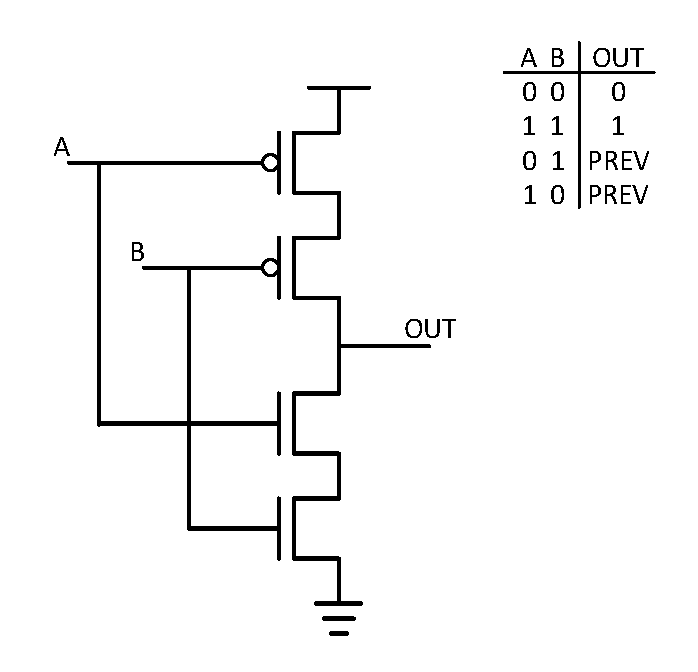
\includegraphics[width=0.75\linewidth]{Figures/C_ele}
	%where an .eps filename suffix will be assumed under latex, 
	%and a .pdf suffix will be assumed for pdflatex; or what has been declared
	%via \DeclareGraphicsExtensions.
	\caption{Muller C-element}
	\label{Cele_fig}
\end{figure}

The most recent and efficient proposed latch is the HSMUF which is proposed in \cite{HSMUF}. This latch uses the TP-DICE structure found in \cite{TPDICE} which is an extended DICE cell with a total of 6 nodes. In the TP-DICE cell, every other node is connected to the input of a 3-input Muller C-element. When a DNU occurs in the worst case, two nodes are set to erroneous value, two nodes are set to high-impedance and two nodes hold the correct value. Since a Muller C-element is placed on the output, the high-impedance and correct nodes hold the output to the correct value. However, a drawback with this design is that it relies on high impedance states for reliability thus the design is non-robust. A common way to mitigate this issue is to place a weak-keeper at the output of the latch as in \ref{HSMUF_fig}. While this design does ensure the output is held, the Muller C-element must be sized such that the driving strength exceeds the that of the keeper. According to our simulations found in Section [REFERENCE RESULTS], the addition of the keeper substantially increases the delay, area and power consumption. 

\begin{figure}[!htbp]
\centering
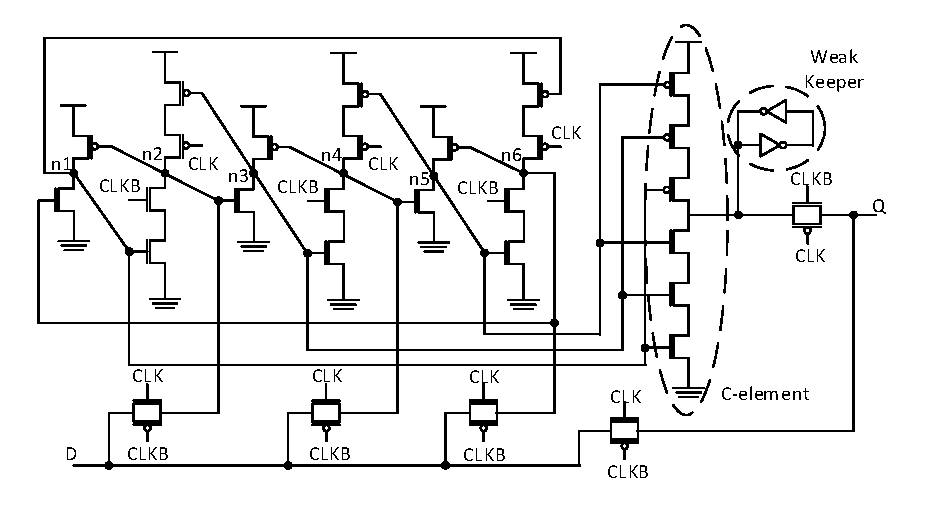
\includegraphics[width=\linewidth]{Figures/HSMUF}
 %where an .eps filename suffix will be assumed under latex, 
 %and a .pdf suffix will be assumed for pdflatex; or what has been declared
 %via \DeclareGraphicsExtensions.
\caption{HSMUF latch \cite{HSMUF} with a weak keeper on the output.}
\label{HSMUF_fig}
\end{figure}
 
It is shown in Section [REFERENCE] that designing a latch such that each node is capable of recovering all nodes allows for the latch to usable in clock gating while also providing lower power, area and delay compared to the C-element approach. As stated in Section \ref{sec:introduction}, latches that are capable of recovering all nodes after an error a called robust. This unique feature is desirable since it leads to more efficient latch designs that can recover from an error. One of the existing DNU-robust design is the DONUT latch proposed in \cite{DONUT} which is the most area efficient design. This latch is based on the combination of four DICE latches creating twelve nodes. Each node is connected to cross-coupled transistors. Since the design is based on the DICE latch, it is able to exploit the recovery feature of the latch. One issue that was discovered during the testing of this latch is that it suffered from excessively high power and delay. It was found that the root of the problem was due to data contention on the data loading lines. To solve this issue, the latch was modified such that the data loading nodes were set to high impedance during the transparent mode. As shown in Section [REFERENCE RESULTS], this modification saved a large amount of power. This design is referred to as the DONUT-M and is given in Fig. \ref{DONUT_M}.

\begin{figure}[!htbp]
	\centering
	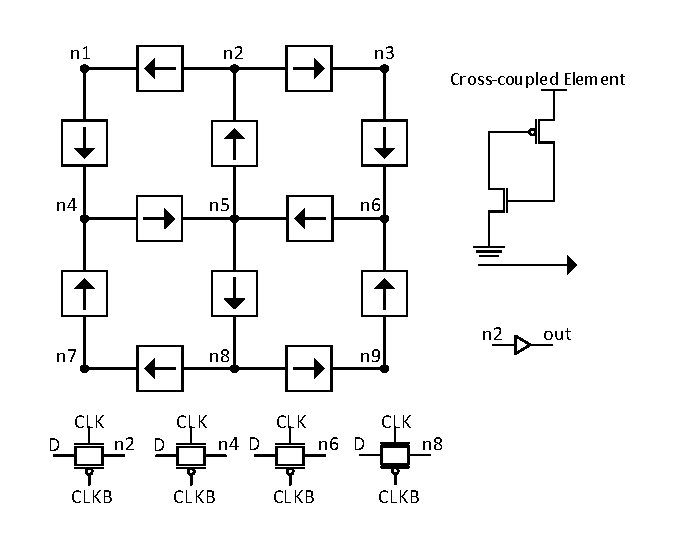
\includegraphics[width=\linewidth]{Figures/DONUT}
	%where an .eps filename suffix will be assumed under latex, 
	%and a .pdf suffix will be assumed for pdflatex; or what has been declared
	%via \DeclareGraphicsExtensions.
	\caption{DONUT latch as proposed in \cite{DONUT}.}
	\label{fig:DONUT}
\end{figure}

\begin{figure}[!htbp]
	\centering
	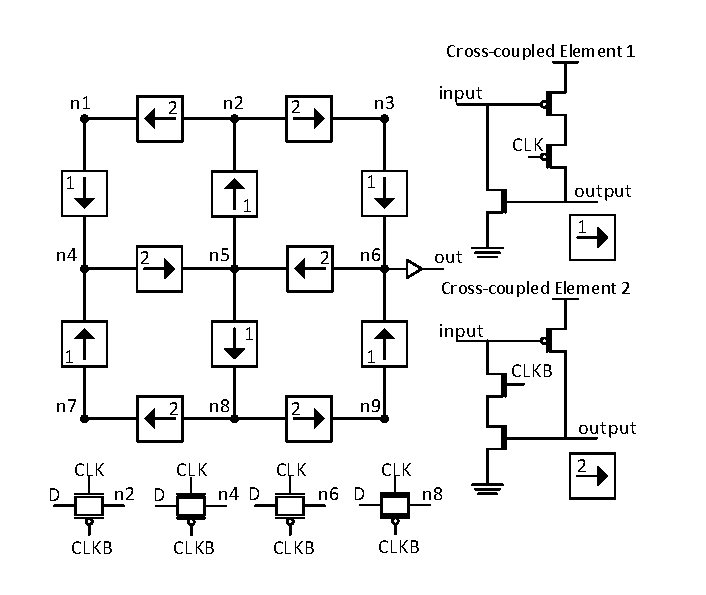
\includegraphics[width=\linewidth]{Figures/ModDONUT}
	%where an .eps filename suffix will be assumed under latex, 
	%and a .pdf suffix will be assumed for pdflatex; or what has been declared
	%via \DeclareGraphicsExtensions.
	\caption{Modified low-power DONUT latch.}
	\label{DONUT_M}
\end{figure}

In addition to DNU tolerant latches, we also investigate the TNU latch. The authors in \cite{Blum2007} propose a latch design that shows limited TNU tolerance. Their design uses eight nodes and eight 2-input C-elements. There are four input signals which are each connected to the output of a C-element to load the data during the transparent mode. In the hold mode, the latch is fully tolerant to a DNU since at least one of the erroneous nodes will be driven by a C-element with error-free inputs. However, when a TNU occurs, the latch is only tolerant if all three errors are on adjacent nodes. 